\section{Experiments}

We conducted several performance tests to measure the throughput and scalability of our system. All these tests were performed in an LAN system called Lattice which has a network bandwidth of 1Gbps. All nodes are Intel(R) Xeon(R) 2.4GHz 4 core duo machines with 1 Gbp of memory. Sample code used for all tests can be found here.

\subsection{Inter node communication}
We used a graph as shown in Figure \ref{ecgGraph} to process ECG signal data. For our solution and Yahoo S4! EventProducer reads a file contains over 7500000 ecg records and push events with multiple threads. Twitter Storm does not allow user threads to push data. So we use the Spout thread to send messages into the system. EventReceiver  receives the ECG events, process them and calculate heart rate interval periodically.  
We execute our system with 1, 2 and 4  EventReceivers for each system and measured the throughput, load average and network bandwidth  for each case. Throughput was measured at the EventProducer calculating total time required to send messages and the total number of messages send. Load average and network bandwidth were measured using top and atop linux commands respectively. Figure \ref{throuput} shows the throughput variation with the number of nodes for all systems. 

\begin{figure}[!t]
        \centering
        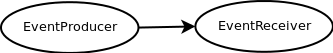
\includegraphics[width=3.0in]{ecgGraph.png}
        \caption{ECG Process Graph}
        \label{ecgGraph}
\end{figure}
\begin{figure}[!t]
        \centering
        \includegraphics[width=3.0in]{throughput.png}
        \caption{Throughput of the systems}
        \label{throuput}
\end{figure}

As shown in the Figure \ref{throuput} our solution out performs Twitter storm and Yahoo S4!. However by looking the Figure \ref{throuput} one might think even our system does not scalable although it perform high. In order to examine the reason behind this we need to look into the network bandwidth and CPU load average values. 
 
Figure \ref{networkandload} shows the network bandwidth usage and the CPU load average at each node. For multiple node scenarios we observed the same values for bandwidth usage and CPU load average at each receiver. Therefore we have taken the average values of them. 

\begin{figure*}[!t]
	\centering
	\subfloat[Network Usage]{\includegraphics[width=3.0in]{network.png}}
	\hfil
	\subfloat[CPU Load Average]{\includegraphics[width=3.0in]{loadaverage.png}}
	\caption{Network usage and CPU Load Average of the System}
	\label{networkandload}
\end{figure*}
 

By looking at the graphs, first it can be observed that our solution utilities all available network bandwidth (98\%) even with two receivers. In only one receiver case, high CPU load average at receiver indicates it has utilized available CPU power. Adding two receivers has increased the CPU power at receiving side utilizing all available network bandwidth. Therefore it can not increase the throughput without increasing network bandwidth although more CPU power available at receiver nodes. Having receiver nodes, we can observe that network bandwidth and CPU load average is reduced at each receiver since load is shared among the receivers. However for other two systems, it neither hits the maximum network bandwidth available nor the full CPU power available at any stage. If a system does not make use of the available resources then adding more resources won't scale up the system. As explained in earlier, our solution utilities all available resources by using parallel tcp connections and having an efficient message parsing technique.

After measuring the throughput we examined the  total amount of extra bytes each system sends to transfer the information from EventProducer to EventReceiver. Our ECGEvent has two double fields called time and value (ecg signal value) and a streamID which is a 4 byte string. So we calculated total bytes to send this information as 20 bytes (16 for two double and 4 for streamID). Then by using the throughput and the bandwidth usage of the system we calculate the total number of bytes each system uses at network layer to send this message. By reducing 20 information bytes we can calculate the over head bytes for each system. Figure \ref{efficiency} compares these numbers.

\begin{figure}[!t]
        \centering
        \includegraphics[width=3.0in]{efficiency.png}

        \caption{Efficiency of Message serialization}
        \label{efficiency}
\end{figure}

As shown in the figure \ref{efficiency} Twitter storm uses a minimum over head while Yahoo S4! performs badly compared to other two. This overhead is due to its usage of  java serializations to serialize data. Then we analyzed to which our solution spends extra 32 bytes. Our solution adds a sequence number (an integer), receiving process id (a 8 byte string for this scenario), sending process id (a 8 byte string for this scenario) to order messages, dispatch the message to correct process and to parse the message at the server. Altogether it adds 26 (serialization format of a string uses two more bytes to keep the string length) extra bytes to each message at application level and other 4 bytes due to tcp over head. This is the trade off we had to pay for improve the parallelism compared to direct one tcp communication per process. 

\subsection{Scalability}
We performed a scalability test for our system using the 3 level graph shown in Figure \ref{multigraph}. The processing data as well as the processing logic were obtained from the Grand Challenge problem of 8th ACM International conference on Distributed Event Based systems. We used the publicly available 500MB of data to generate the events. 

\begin{figure}[!t]
        \centering
        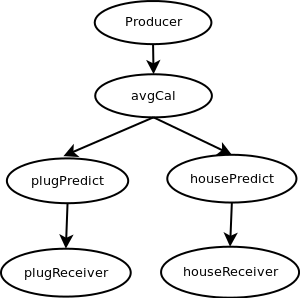
\includegraphics[width=3.0in]{multigraph.png}
        \caption{Multilevel Node Graph}
        \label{multigraph}
\end{figure}

This application predicts load averages using the previous values and a given machine learning algorithm. We implement this logic using nodes as shown in the Figure \ref{multigraph}. First producer reads the data file and send events to the avgCal node which calculate the last minite average and send the same event to both plugPredict and housePredict processors. Both plugPredict and housePredict processors predict the next values and send events to receivers. The original problem only requires to send those prediction events in 30s intervals. But we send a prediction event fore each messages to observe how the system works with high load.
 
As in the earlier case we conduct our experiments using one producer and multiplying the other processing nodes by 1, 2 and 4 times to measure the throughput increase at the producer. We ran each node in a separate machine so that our receiver configurations used 5, 10, 15 machines respectively. We measured the throughput,  network bandwidth and the CPU load average at the producer to examine the scalability of the system. Since the one receiver unit throughput greater than that of the storm one node scenario we only used our system for this experiment.  Results are shown in the Figure \ref{scalability}.

%\begin{figure}
%        \centering
%        \begin{subfigure}[b]{0.45\textwidth}
%                \includegraphics[width=\textwidth]{throughputs.png}
%        \end{subfigure}
%        \begin{subfigure}[b]{0.45\textwidth}
%                \includegraphics[width=\textwidth]{networkps.png}
%        \end{subfigure}
%        \begin{subfigure}[b]{0.45\textwidth}
%                \includegraphics[width=\textwidth]{networks.png}
%        \end{subfigure}
%        \begin{subfigure}[b]{0.45\textwidth}
%                \includegraphics[width=\textwidth]{loadaverages.png}
%        \end{subfigure}
%        \caption{Scalability of the System}
%        \label{scalability}
%\end{figure} 

\begin{figure*}[!t]
        \centering
        \subfloat[Throughput]{\includegraphics[width=3.0in]{throughputs.png}}
        \hfil
        \subfloat[Network Usage]{\includegraphics[width=3.0in]{networkps.png}}
        \hfil
        \subfloat[Network Usage Bandwidth]{\includegraphics[width=3.0in]{networks.png}}
        \hfil
        \subfloat[CPU Load Average]{\includegraphics[width=3.0in]{loadaverages.png}}
        \caption{Scalability of the System}
        \label{scalability}
\end{figure*}


For one receiver unit case, we observed very high load average and network bandwidth usage at avgCal node since it send messages to two nodes. Then as shown in the figure \ref{scalability} we could linerly scale up the system by adding more receiver units to add more cpu power to system. When increasing the receiver units, we can observe throughput of the system increases proportional to number of receiving units. CPU load average of 13 at the producer indicates it has utilized all available CPU power and we need to add more producers to scale this system further up. 


